\documentclass[]{standalone}
\usepackage{tikz}
\begin{document}
  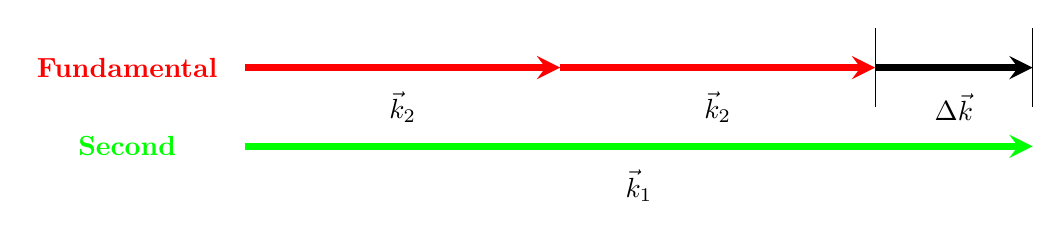
\begin{tikzpicture}
	\node[color = green] at (-1.5,0) (fundamental) {\textbf{Second}};
	\draw[->,>=stealth, line width = 2.6pt, color = green] (0,0) -- (10,0);
	\node[color = red] at (-1.5,1) (fundamental) {\textbf{Fundamental}};
	\node[] at (5,-.5) (k1) {\textbf{$\vec k_1$}};
	\draw[->,>=stealth, line width = 2.6pt, color = red] (0,1) -- (4,1);
	\draw[->,>=stealth, line width = 2.6pt, color = red] (4,1) -- (8,1);
	\node[] at (2,.5) (k2) {\textbf{$\vec k_2$}};
	\node[] at (6,.5) (k2a) {\textbf{$\vec k_2$}};
	\draw[] (8,1.5) -- (8,.5);
	\draw[] (10,1.5) -- (10,.5);
	\draw[->,>=stealth, line width = 2.6pt] (8,1) -- (10,1);
	\node at (9,.5) (delk) {\textbf{$\Delta \vec k$}};
  \end{tikzpicture}
\end{document}
